\documentclass[10pt,aspectratio=169,dvipsnames]{beamer}
\usetheme[]{Berlin}

\setbeamertemplate{footline}{
  \usebeamercolor[fg]{framesource}%
  \usebeamerfont{page number in head}%
  \hspace{0.2cm}
  \small \insertframenumber
  \vspace{0.2cm}
  \doclicenseIcon
  \hfill
  
\includegraphics[height=0.8cm]{logos/tub_logo.pdf}
  \hspace{0.2cm}
}

\setbeamercovered{transparent}

\setbeamertemplate{footline}[
 myframe number]

% PACKAGES
\usepackage[absolute,overlay]{textpos}
\usepackage[utf8]{inputenc}
\usepackage[official]{eurosym}
\usepackage{booktabs}
\usepackage{parskip}
\usepackage{bm}
\usepackage{tikz}
\usepackage{adjustbox}

\usepackage[
    type={CC},
    modifier={by},
    version={4.0},
]{doclicense}

% HYPERREFERENCES
\usepackage{hyperref}
\hypersetup{
	colorlinks=true,
	citecolor=tub-blue,
	linkcolor=tub-blue,
	urlcolor=tub-blue
}

\usepackage[sfdefault]{roboto}
\usepackage[normalem]{ulem}
\usepackage{multicol}

% GRAPHICS	
\graphicspath{
    {graphics/},
    {../workflow/notebooks/figures} % study results
  }
\DeclareGraphicsExtensions{.pdf,.jpeg,.png,.jpg}

% FORMATTING
\setlength{\parskip}{6pt}
\linespread{1.1}
\newcommand{\seprule}{\par\noindent\textcolor{black!25}{\rule{\textwidth}{0.4pt}}}

% SOURCES
\setbeamercolor{framesource}{fg=gray}
\setbeamerfont{framesource}{size=\tiny}
\newcommand{\source}[1]{\begin{textblock*}{10cm}(3.6cm,8.25cm)
    \begin{beamercolorbox}[ht=0.5cm,right]{framesource}
        \usebeamerfont{framesource}\usebeamercolor[fg]{framesource} Source: {#1}
    \end{beamercolorbox}
\end{textblock*}}

% REFERENCES
% \usepackage[style=nature, doi=true, maxcitenames=3]{biblatex}
% \bibliography{bibliography}
% \renewcommand*{\bibfont}{\footnotesize}

% COLOR TEXT
\newcommand{\bl}[1]{\textcolor{tub-blue}{#1}}
\newcommand{\gr}[1]{\textcolor{tub-green}{#1}}
\newcommand{\rd}[1]{\textcolor{tub-red}{#1}}
\newcommand{\yl}[1]{\textcolor{tub-yellow}{#1}}
% \newcommand{\org}[1]{\textcolor{tub-orange}{#1}}
\newcommand{\cb}[1]{\colorbox{gray!20}{#1}}

\usepackage{array}% https://ctan.org/pkg/array
\makeatletter
\g@addto@macro{\endtabular}{\rowfont{}}% Clear row font
\makeatother
\newcommand{\rowfonttype}{}% Current row font
\newcommand{\rowfont}[1]{% Set current row font
   \gdef\rowfonttype{#1}#1%
}
\newcolumntype{L}{>{\rowfonttype}l}
\newcolumntype{R}{>{\rowfonttype}r}

% FONT
%\usepackage{utopia}

% REFERENCES
%\usepackage[backend=biber,style=authoryear-comp]{biblatex}
%\bibliography{references.bib}

% TITLE PAGE
\title{
  ISEASA\\1st International Symposium on Energy System Analysis 
}
\vspace*{-.5cm}

% \author{STRIse}
\institute[Technische Universität Berlin] % (optional, but mostly needed)
{ 
  \normalsize
  \alert{Resilient strategies for the European energy system} \\
  \alert{A case study on 2030 EU policy targets} \\
  \footnotesize
  \textbf{Bobby Xiong}\\
  \href{mailto:xiong@tu-berlin.de}{xiong@tu-berlin.de} \\
  % Department of Digital Transformation in Energy Systems \\
  Technische Universität Berlin, Germany \\

  \vspace{0.2cm}

  November 11, 2024
}

\date{}

\subject{Recent Research with PyPSA-Eur}

\titlegraphic{%
\vspace{-1cm}

\includegraphics[height=1cm,clip=true]{logos/cetp_logo.png}
\hspace{0.5cm}
\includegraphics[height=1cm,clip=true]{logos/ensys_short_logo.pdf}
\hspace{0.5cm}
\includegraphics[trim=0 0cm 0 0cm,height=1cm,clip=true]{logos/tub_logo.pdf}
\hspace{0.5cm}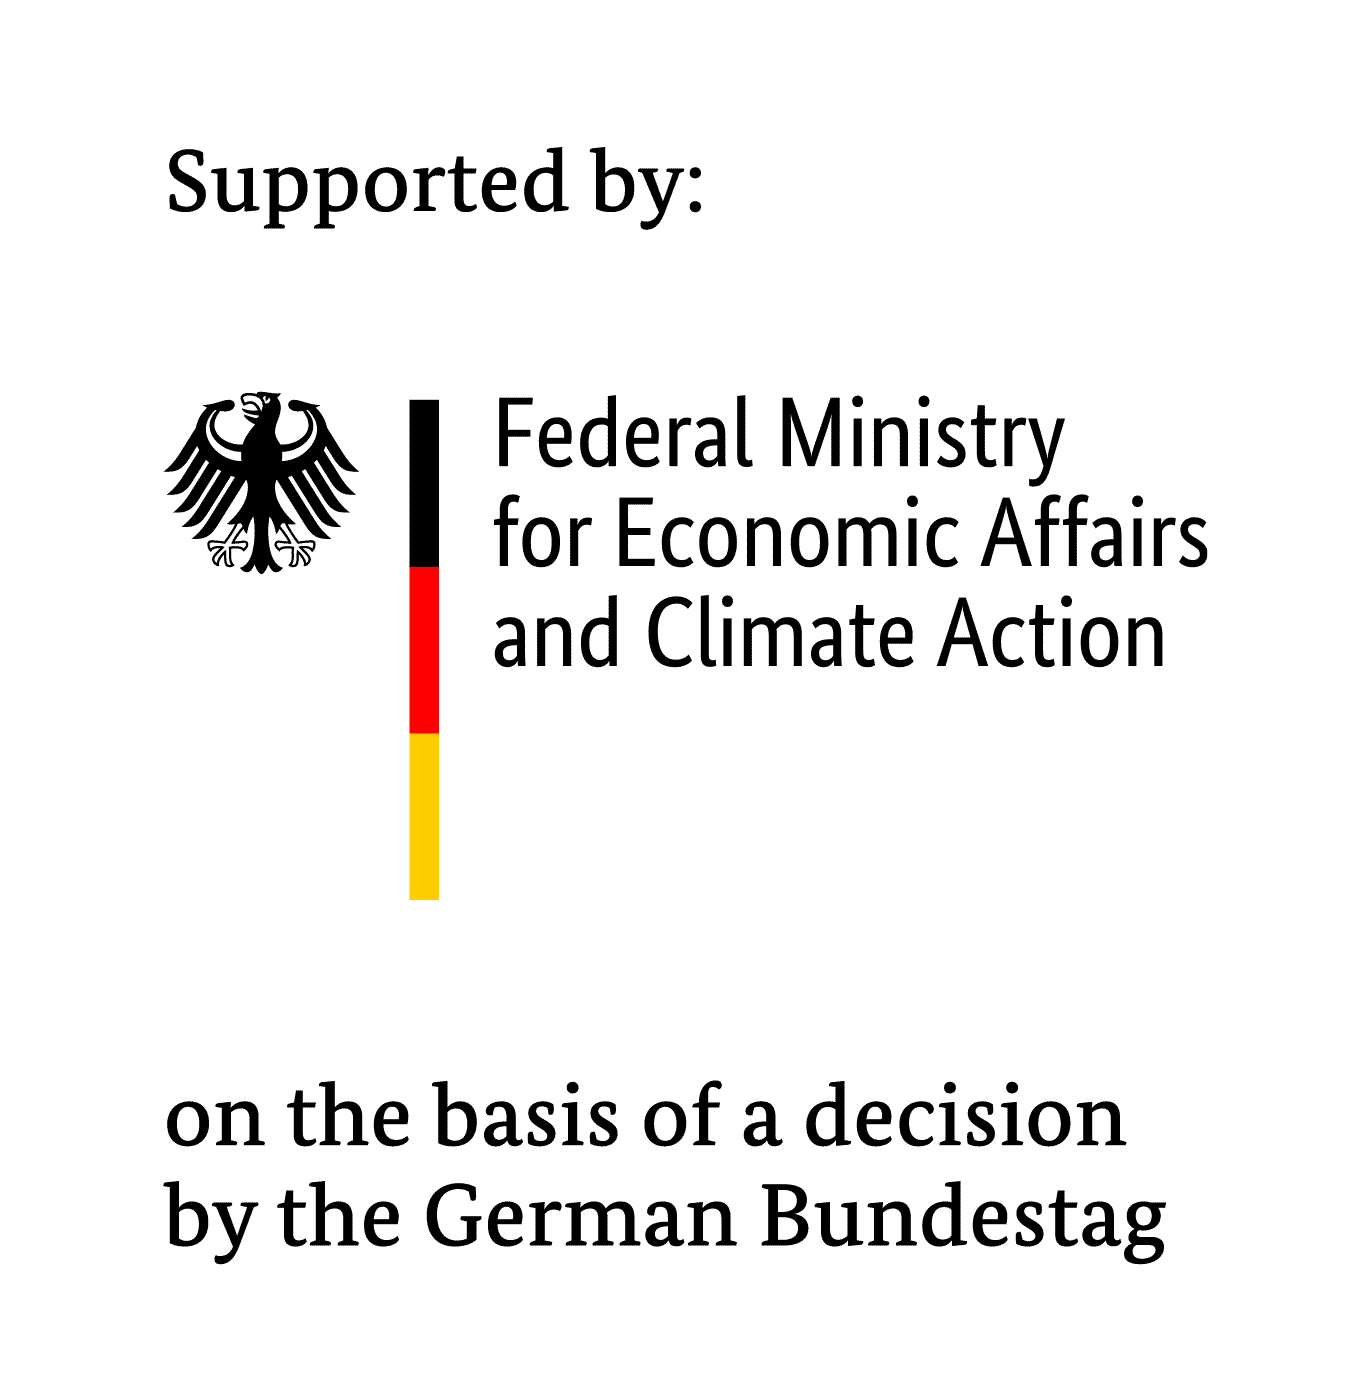
\includegraphics[trim=0.2cm 0.6cm 0.6cm 0.2cm,height=1.1cm,clip=true]{logos/bmwk_en_logo.png}
}


\begin{document}

\addtocounter{framenumber}{-1}
{
  \setbeamertemplate{footline}{
    \usebeamercolor[fg]{framesource}%
    \usebeamerfont{page number in head}%
    \begin{center}
      \Large
      \doclicenseIcon
      \vspace{0.4cm}
    \end{center}
  } 
  \maketitle
}

\section{Introduction}


\begin{frame}{RESILIENT project partners}
  \centering
  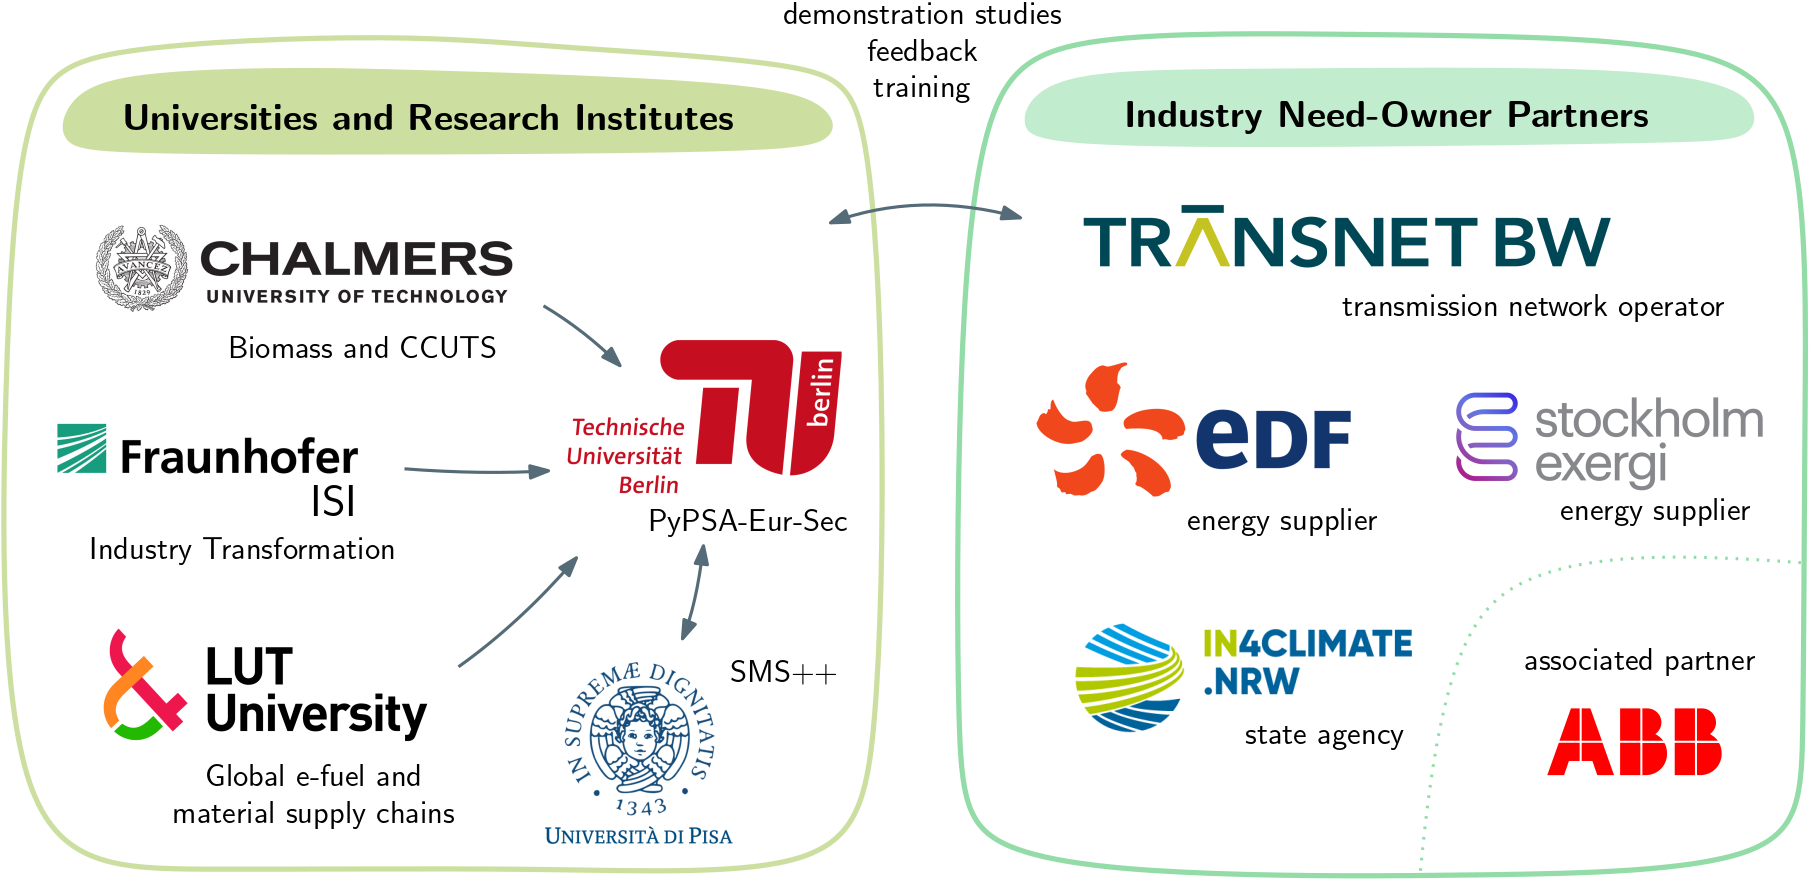
\includegraphics[width=0.85\textwidth]{other/resilient_partners}
  
  \footnotesize
  Funded via \alert{CETPartnership 2022} Call -- \alert{BMWK} for all German partners.

  \source{\url{https://resilient-project.github.io/}}
\end{frame}

% \begin{frame}{Work Plan}
%   \centering
%   \includegraphics[width=0.8\textwidth]{resilient-v3.1}
% \end{frame}

\begin{frame}{PyPSA-Eur: An open-source, sector-coupled model for Europe}
  \begin{columns}
    \begin{column}{0.45\textwidth}
      \footnotesize
      \begin{itemize}
        \setlength\itemsep{.8em}
        \item Spatially and temporally highly linear optimisation model that covers the European continent,
        \item Built on top of the open-source toolbox PyPSA,
        \item Includes stock of existing power plants, renewable potentials, availability time series,
        \item Covers the electricity high-voltage grid from AC 220 kV to 750 kV (UA) and DC 150 kV upwards, option to include planned transmission projects (TYNDP and German NEP),
        \item Maintained by the Department of Digital Transformation in Energy Systems at TU Berlin.
      \end{itemize}
    \end{column}
    \begin{column}{0.55\textwidth}
      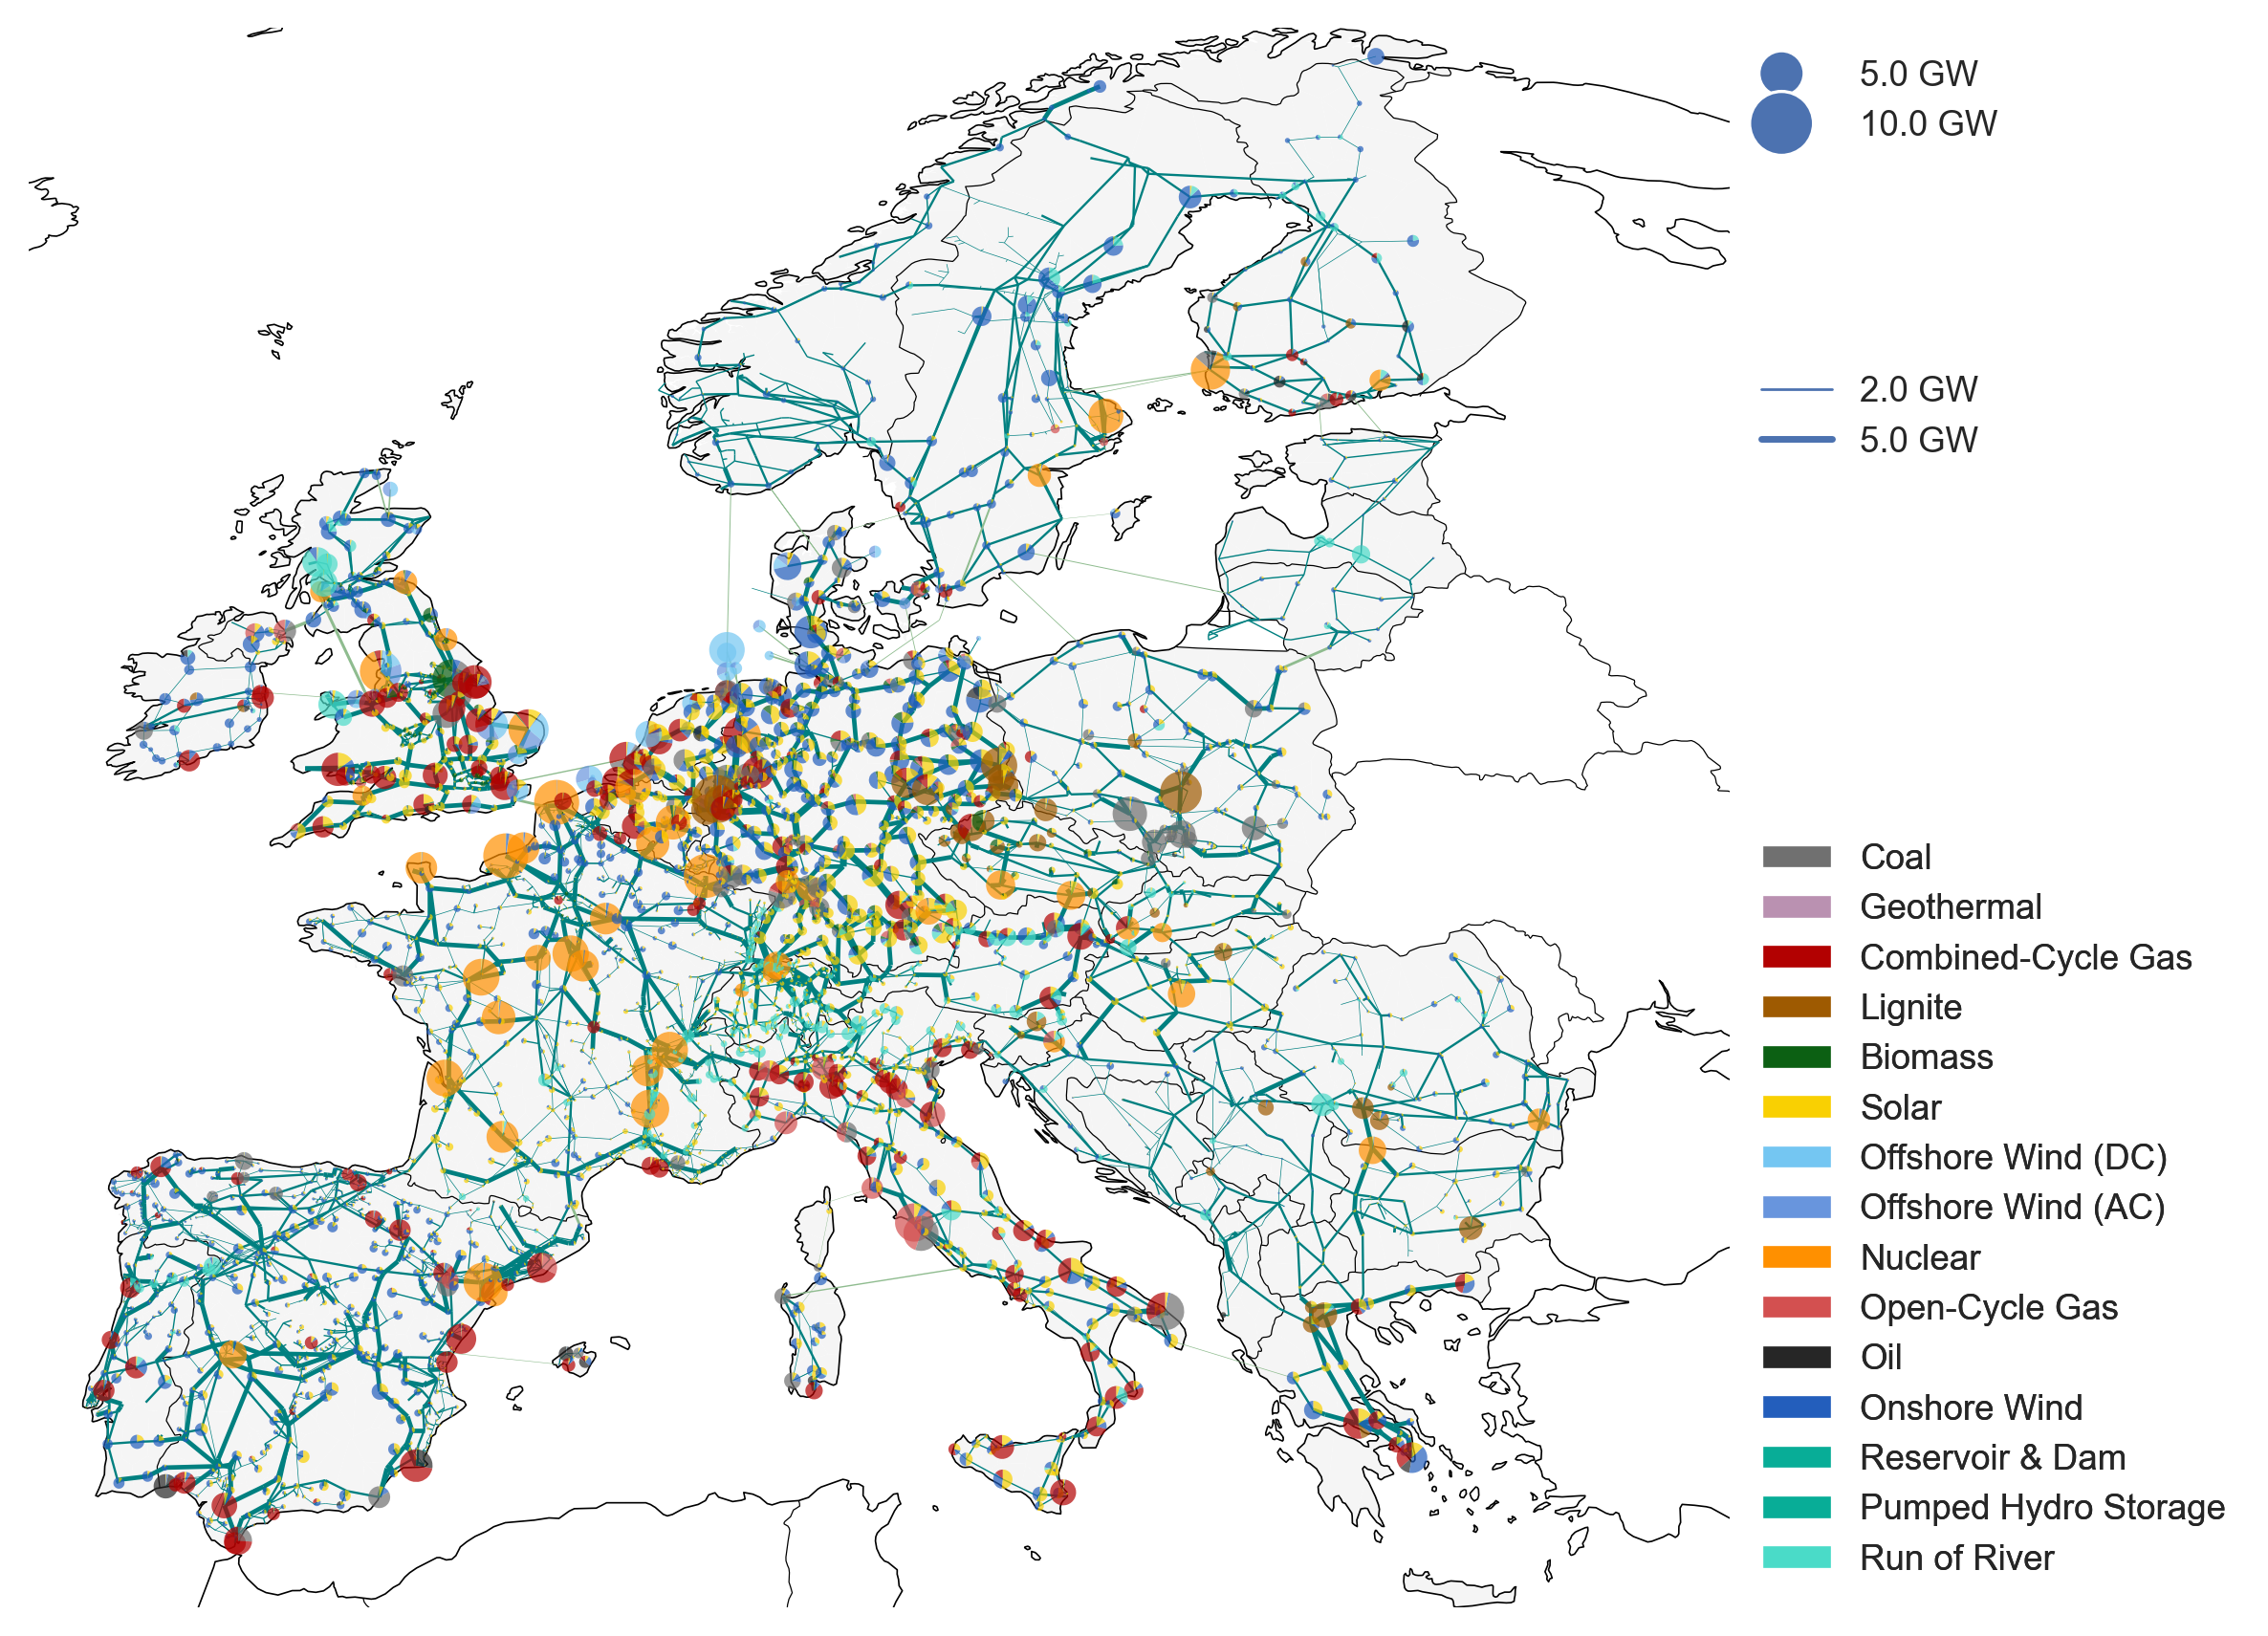
\includegraphics[width=1\textwidth]{other/pypsa_eur_elec}
    \end{column}
  \end{columns}

  \source{\url{https://pypsa-eur.readthedocs.io}}
\end{frame}

\begin{frame}{Selection of planned model developments}
  \begin{columns}[T] % align columns
    \begin{column}{.5\textwidth}
        \begin{minipage}[t][.45\textheight]{\linewidth}
            \begin{alertblock}{Computational methods for uncertainties}
                \begin{itemize}
                  \item decomposition techniques
                  \item large-scale stochastic optimisation
                  \item \textbf{test robustness of system}
                  \item using SMS++ framework
                \end{itemize}
            \end{alertblock}
        \end{minipage}
        
        \vspace{0.03\textheight} % separation between the boxes
        
        \begin{minipage}[t][.45\textheight]{\linewidth}
            \begin{alertblock}{Industry transformation (FORECAST)}
              \begin{itemize}
                \item fuel and process switching
                \item industry relocation
                \item carbon sources and feedstocks
                \item data on stock \& investment cycles
                \item new technologies (oxyfuel cement, etc.)
              \end{itemize}
            \end{alertblock}
        \end{minipage}
    \end{column}
    
    \begin{column}{.5\textwidth}
        \begin{minipage}[t][.45\textheight]{\linewidth}
            \begin{alertblock}{Carbon management and biomass usage}
              \begin{itemize}
                \item \textbf{CO$_2$ network}
                \item \textbf{CO$_2$ sequestration potentials}
                \item circular carbon economy and recycling
                \item biomass usage options
              \end{itemize}
            \end{alertblock}
        \end{minipage}
        
        \vspace{0.03\textheight} % separation between the boxes
        
        \begin{minipage}[t][.45\textheight]{\linewidth}
            \begin{alertblock}{Global green fuel and material markets}
              \begin{itemize}
                \item \textbf{imports of green energy and materials}
                \item \textbf{effects on European infrastructure}
                \item restructuring of value chains
                \item risks (geopolitical, technological, etc.)
              \end{itemize}
            \end{alertblock}
        \end{minipage}
    \end{column}
\end{columns}
\end{frame}

\section{Case study: PCI/PMI + 2030 targets}

\begin{frame}{Case study: Motivation}
  
  Blabla

  \begin{multicols}{2}
  \begin{itemize}
    \item target 1
  \end{itemize}
  \end{multicols}

  \source{Neumann, Zeyen, Victoria, Brown, 2023; \url{https://doi.org/10.1016/j.joule.2023.06.016}}
\end{frame}

\begin{frame}{Case study: Model setup}
  \begin{columns}
    \begin{column}{0.55\textwidth}
      \footnotesize
      \begin{itemize}
        \setlength\itemsep{.8em}
        \item Including sectors \alert{power, heat, transport, industry, agriculture}
        \item Minimising \alert{total system costs} (investment and operation) for the target
        \item \alert{Co-optimising} generation, transmission, storage, and power-to-X conversion
        \item Resolving 34 countries to \alert{90 regions} at \alert{3-hourly} temporal resolution
        \item Implementing \alert{PCI/PMI} hydrogen and carbon infrastructure projects as well as key \alert{2030 targets}:
        \vspace{0.1cm}
        \begin{itemize}
          \scriptsize
          \item 55 \% emission reduction (\alert{Fit for 55})
          \item 10 Mt p.a. production of hydrogen (\alert{REPowerEU})
          \item 50 Mt p.a. of CO$_2$ sequestration (\alert{Net-Zero Industry Act})
        \end{itemize}
      \end{itemize}
    \end{column}
    \begin{column}{0.45\textwidth}
      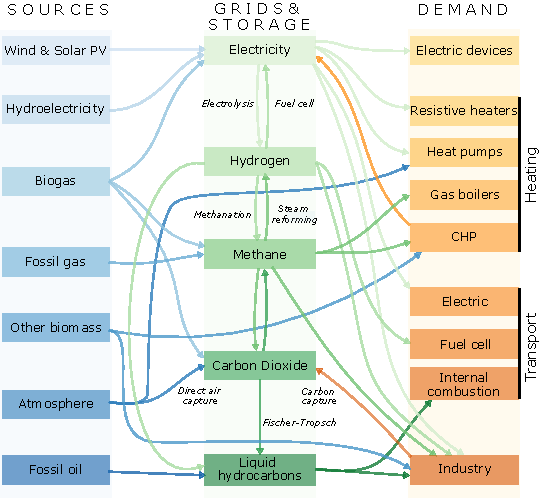
\includegraphics[width=0.95\textwidth]{other/multisector_diagram}
    \end{column}
  \end{columns}
  \source{\url{https://pypsa-eur.readthedocs.io}}
\end{frame}

\begin{frame}{Case study: Overview of PCI-PMI H$_2$ and CO$_2$ infrastructure}

  \begin{columns}
    \begin{column}{0.5\textwidth}
      \footnotesize
      \begin{itemize}
        \setlength\itemsep{.8em}
        \item Baseline scenario incorporates \alert{PCI/PMI} projects for \alert{H$_2$} and \alert{CO$_2$} infrastructure, including pipelines, storages (H$_2$) and sequestration sites (CO$_2$), commissioned by 2030
        \item Total CO$_2$ sequestration potential sums up to \alert{75 Mt p.a.}, mostly located in the North Sea
        \item Total H$_2$ storage capacity sums up to \alert{977 GWh}
      \end{itemize}
    \end{column}
    \begin{column}{0.5\textwidth}
      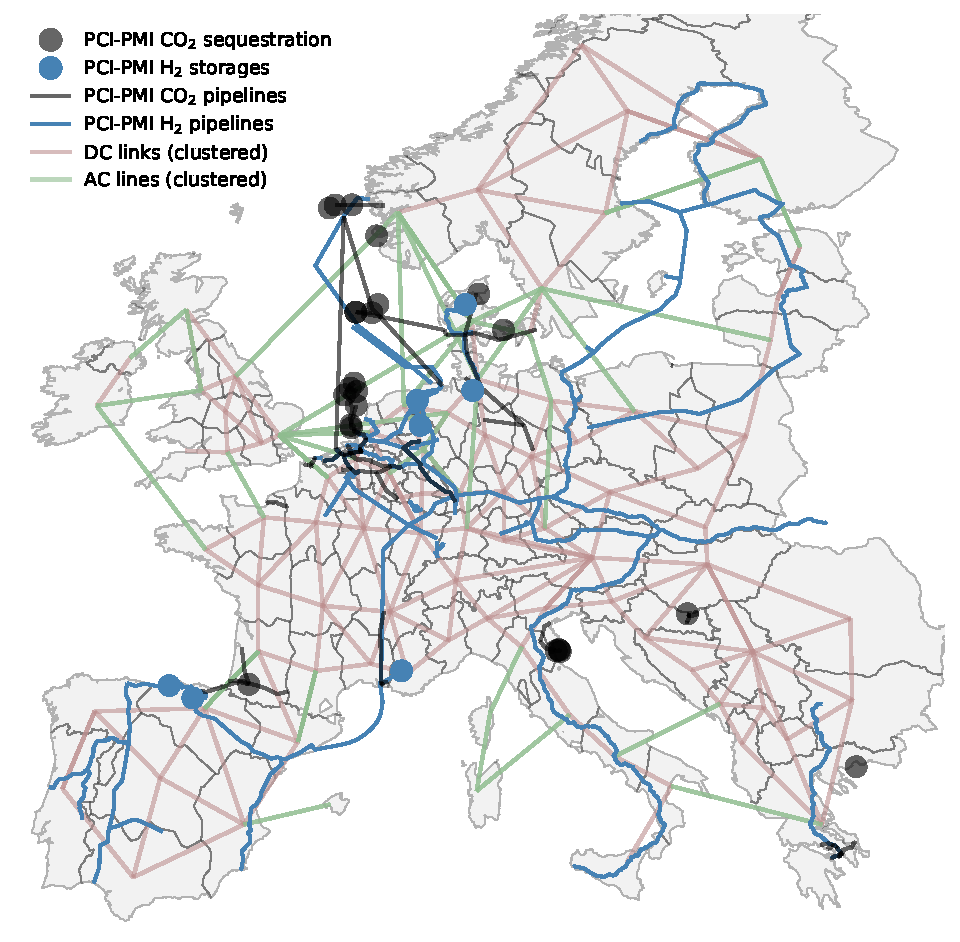
\includegraphics[width=\textwidth]{pci_pmi_projects_map}
    \end{column}
  \end{columns}
  \source{Own illustration based on data extracted from \url{https://ec.europa.eu/energy/infrastructure/transparency_platform/map-viewer}}
\end{frame} 

\section{First results}

\begin{frame}{First results}
  
  \begin{columns}
    \begin{column}{0.2\textwidth}
      \footnotesize
      \begin{itemize}
        \setlength\itemsep{.8em}
        \item test
      \end{itemize}
    \end{column}
    \begin{column}{0.8\textwidth}
      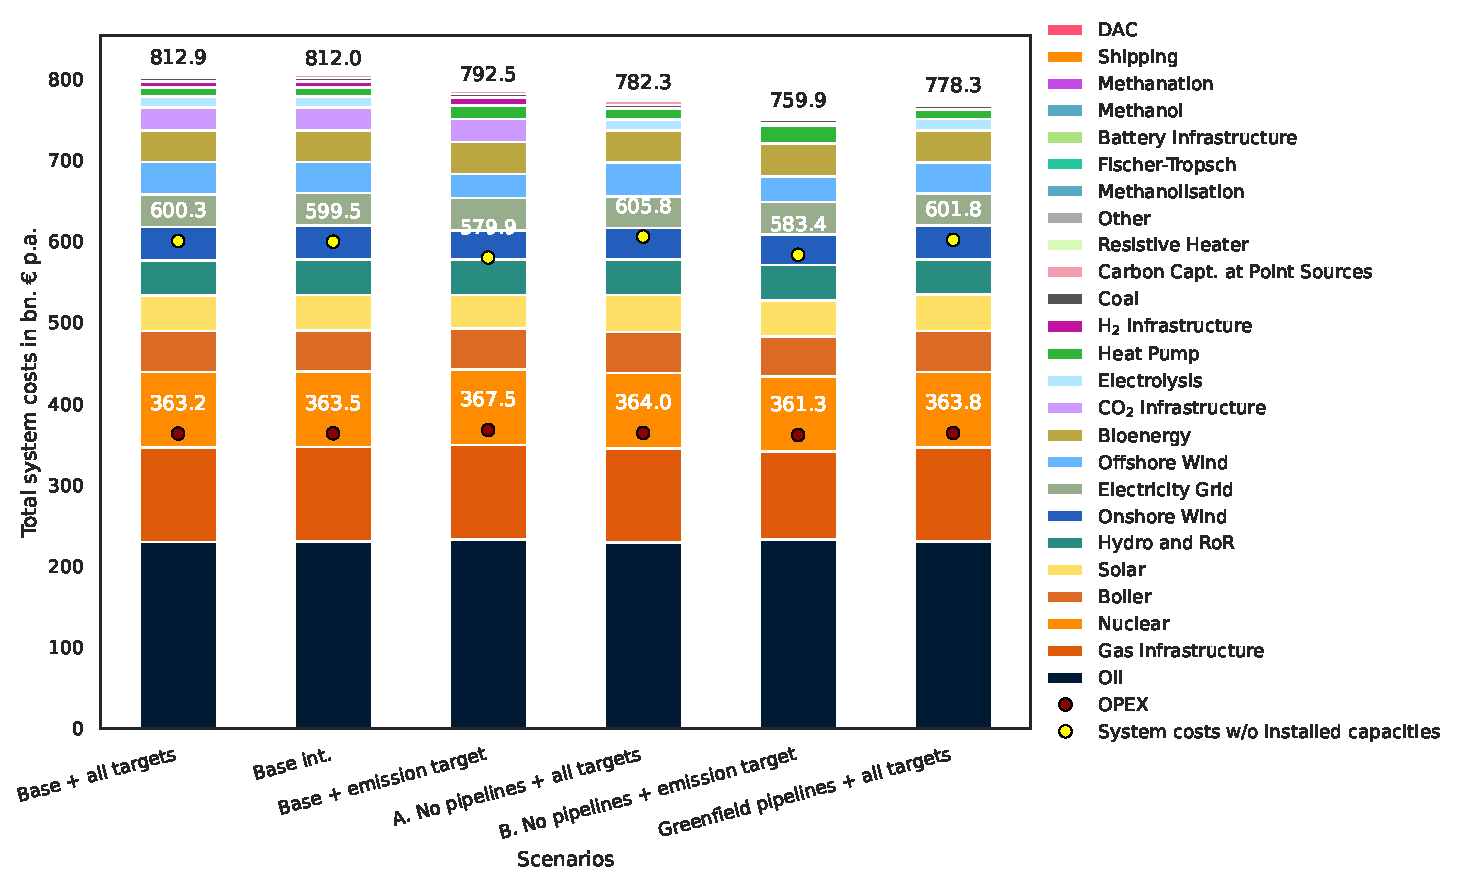
\includegraphics[width=\textwidth]{system_costs}
    \end{column}
  \end{columns}

  \source{Own illustration based on first results}

\end{frame}

\begin{frame}{Case study: First takeaways}
  \footnotesize
  \begin{enumerate}
    \setlength\itemsep{1em}

    \item Imports of green energy could reduce cost of European net-zero system
      \alert{by 1-14\%}.
  
    \item \alert{Diminishing returns} for larger import volumes; \alert{preference} for steel, MeOH and H$_2$.

    \item Infrastructure policy needs \alert{coordination} with import strategy \& carbon management.
  
    \item Protect against interannual weather variability, e.g.~with \alert{(green) fuel reserves}.

    \item Maneuvering space to accommodate non-cost factors: \alert{geopolitics},
    \alert{reuse} of infrastructure, \alert{resilience} of supply chains,
    diversification, and reduced land usage..

    
  \end{enumerate}

\end{frame}

\section{Outlook}
\begin{frame}{Outlook}
  \begin{itemize}
    \item Add all PCI/PMI projects, including hybrid offshore interconnection projects (energy islands), electricity storages, etc.
    \item  
  \end{itemize}
\end{frame}

% Appendix

\section{Appendix}


\begin{frame}{\textbf{Appendix}}
\end{frame}

\begin{frame}{\textbf{Why H$_2$?} Most H$_2$ is used for derivative fuels and chemicals!}
  
  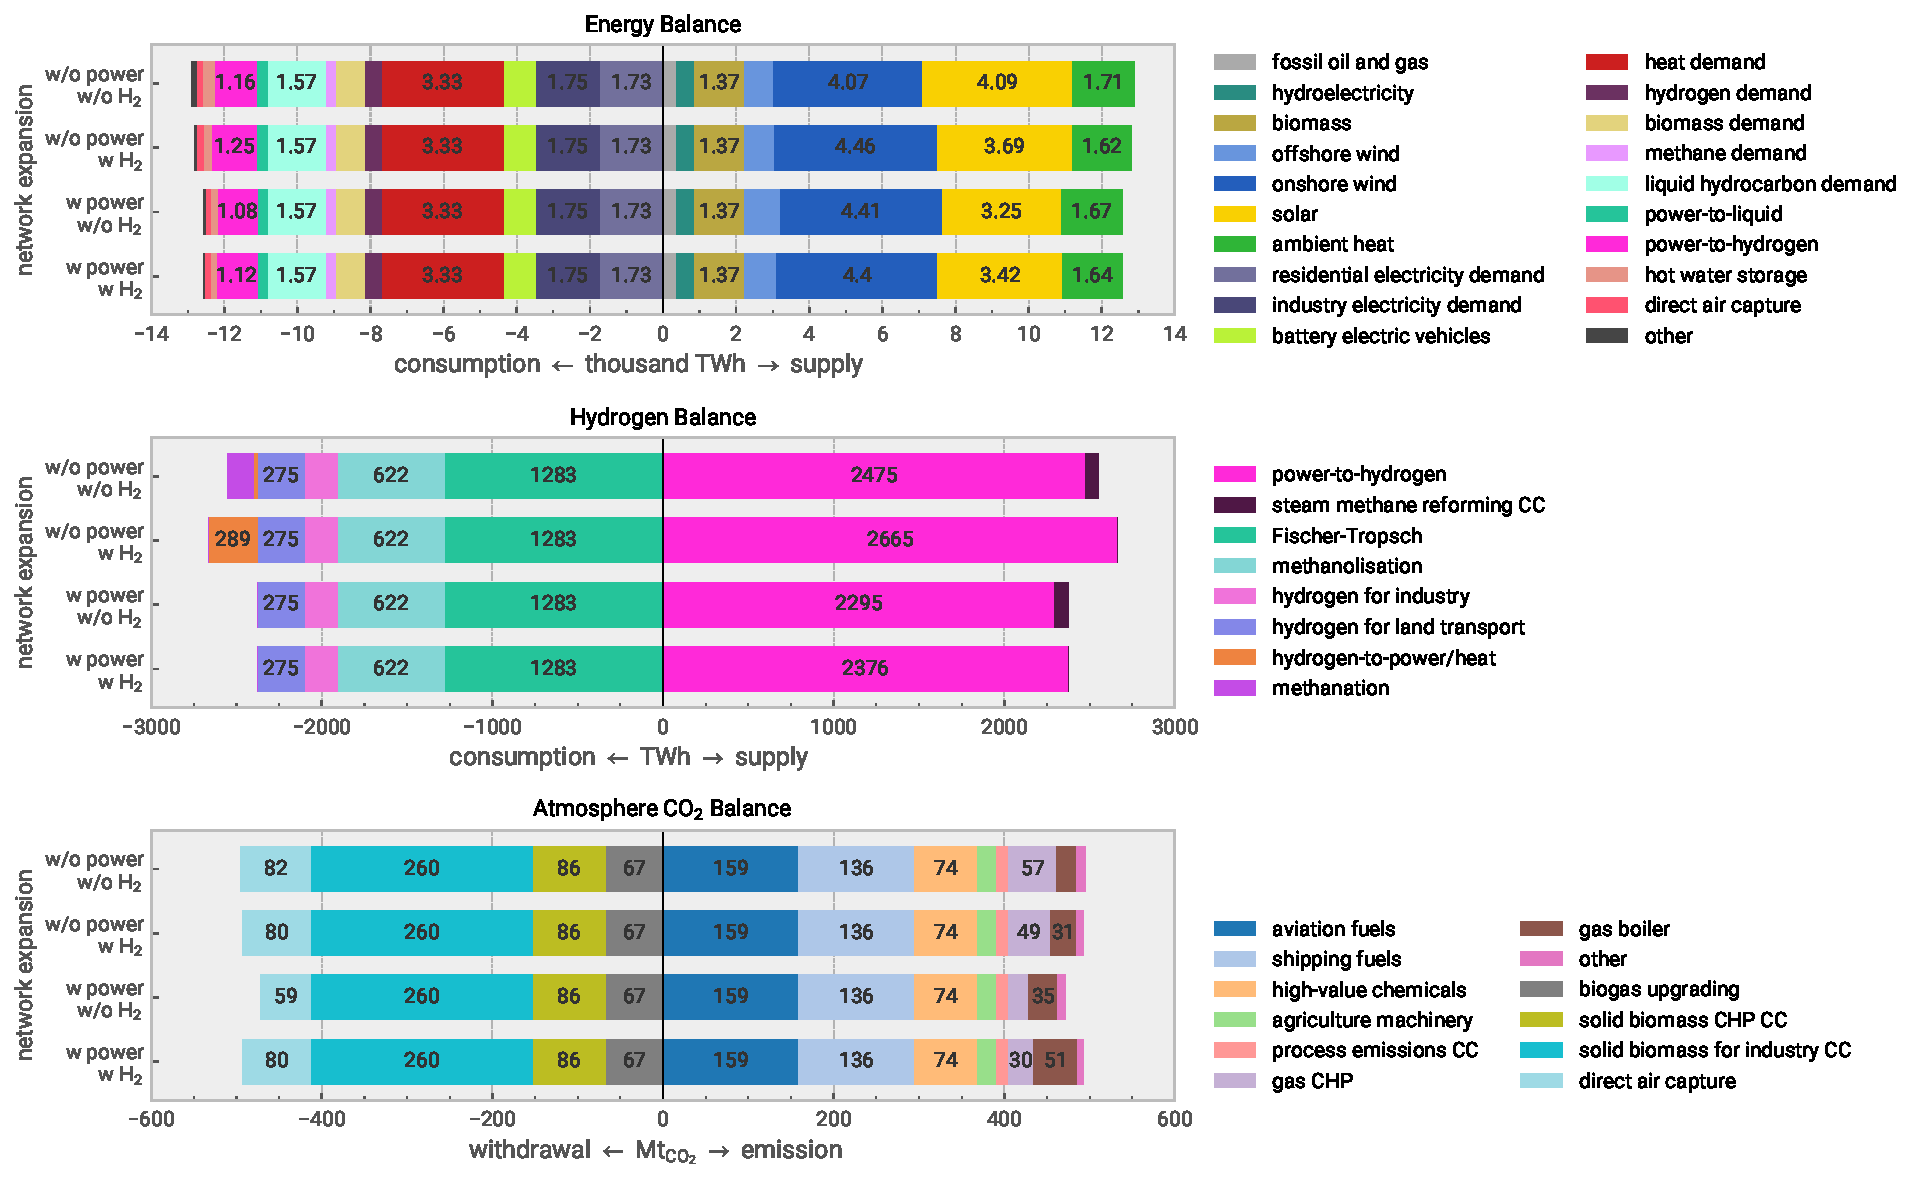
\includegraphics[width=1.2\textwidth, trim=0cm 6.6cm 0cm 6.6cm, clip]{other/hydrogen_balance.pdf}

  Mostly \alert{green electrolytic hydrogen supply}. \alert{Few direct uses of hydrogen} in the energy system, but it is
  used to synthesise other fuels and chemicals:

  \begin{multicols}{2}
  \begin{itemize}
    \item ammonia for fertilizers
    \item direct reduced iron for steelmaking
    \item shipping and aviation fuels
    \item precursor to high-value chemicals
    \item backup heat and power supply
    \item some heavy duty land transport
  \end{itemize}
  \end{multicols}

  \source{Neumann, Zeyen, Victoria, Brown, 2023; \url{https://doi.org/10.1016/j.joule.2023.06.016}}
\end{frame}

\begin{frame}{Transporting \textbf{CO$_2$ to H$_2$} or transporting \textbf{H$_2$ to CO$_2$}?}
  
  \centering
  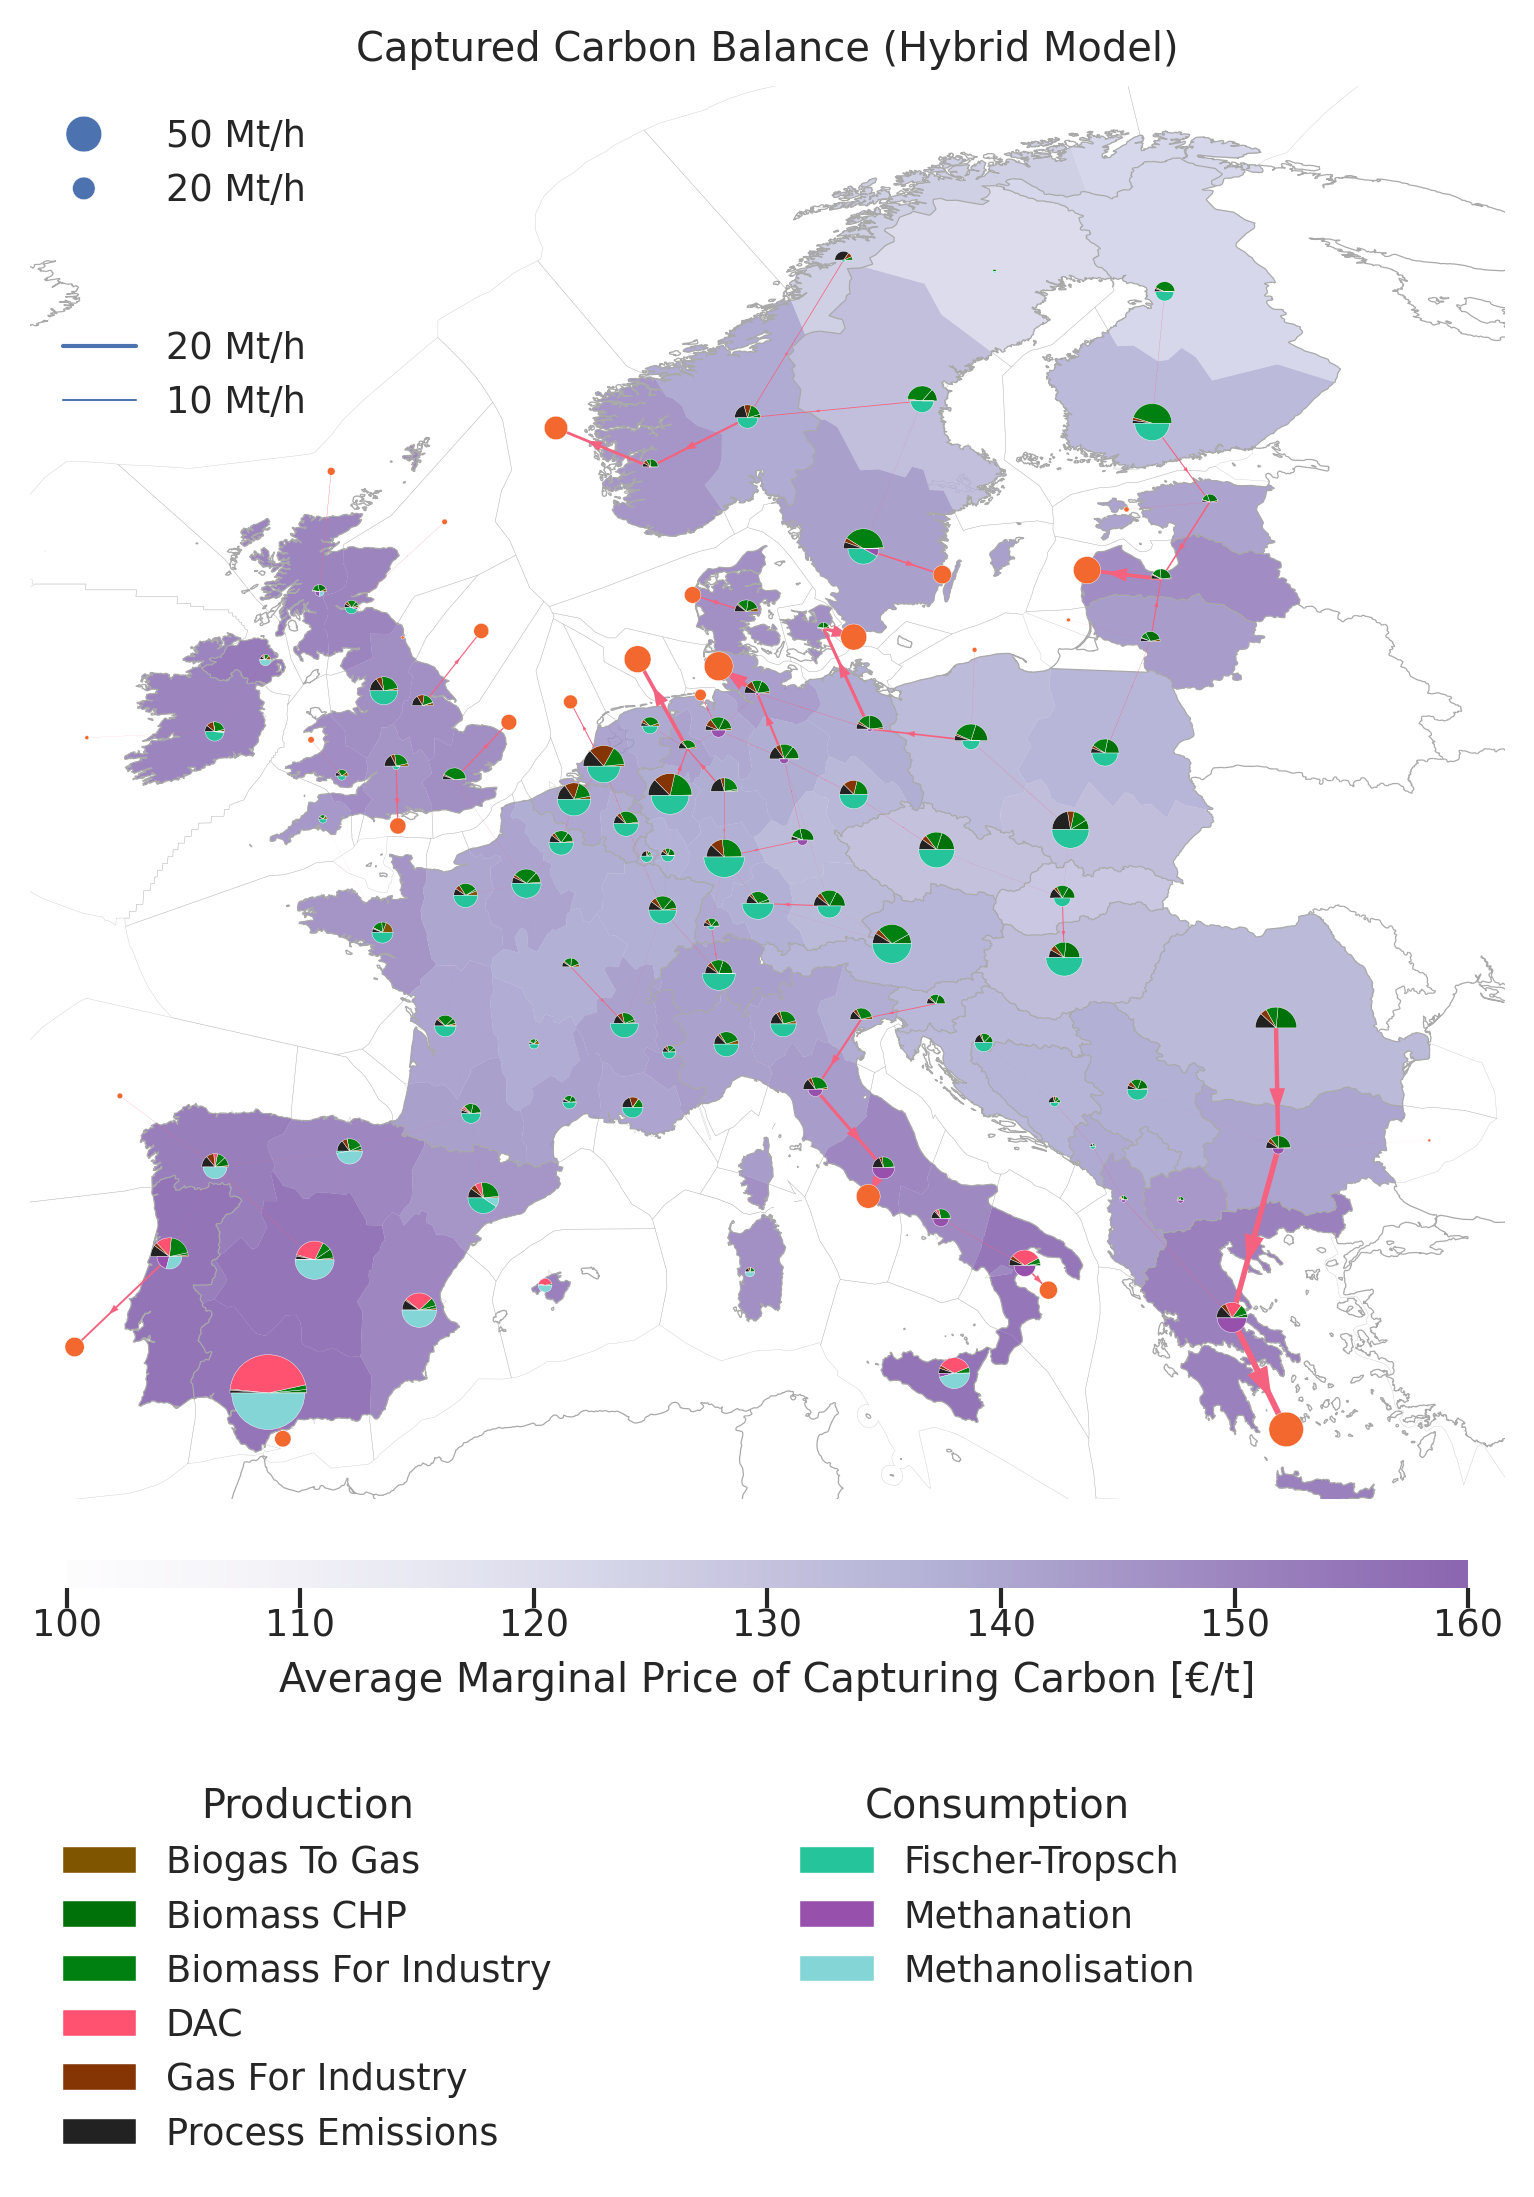
\includegraphics[width=0.35\textwidth]{other/carbon_networks_balance_map_carbon}
  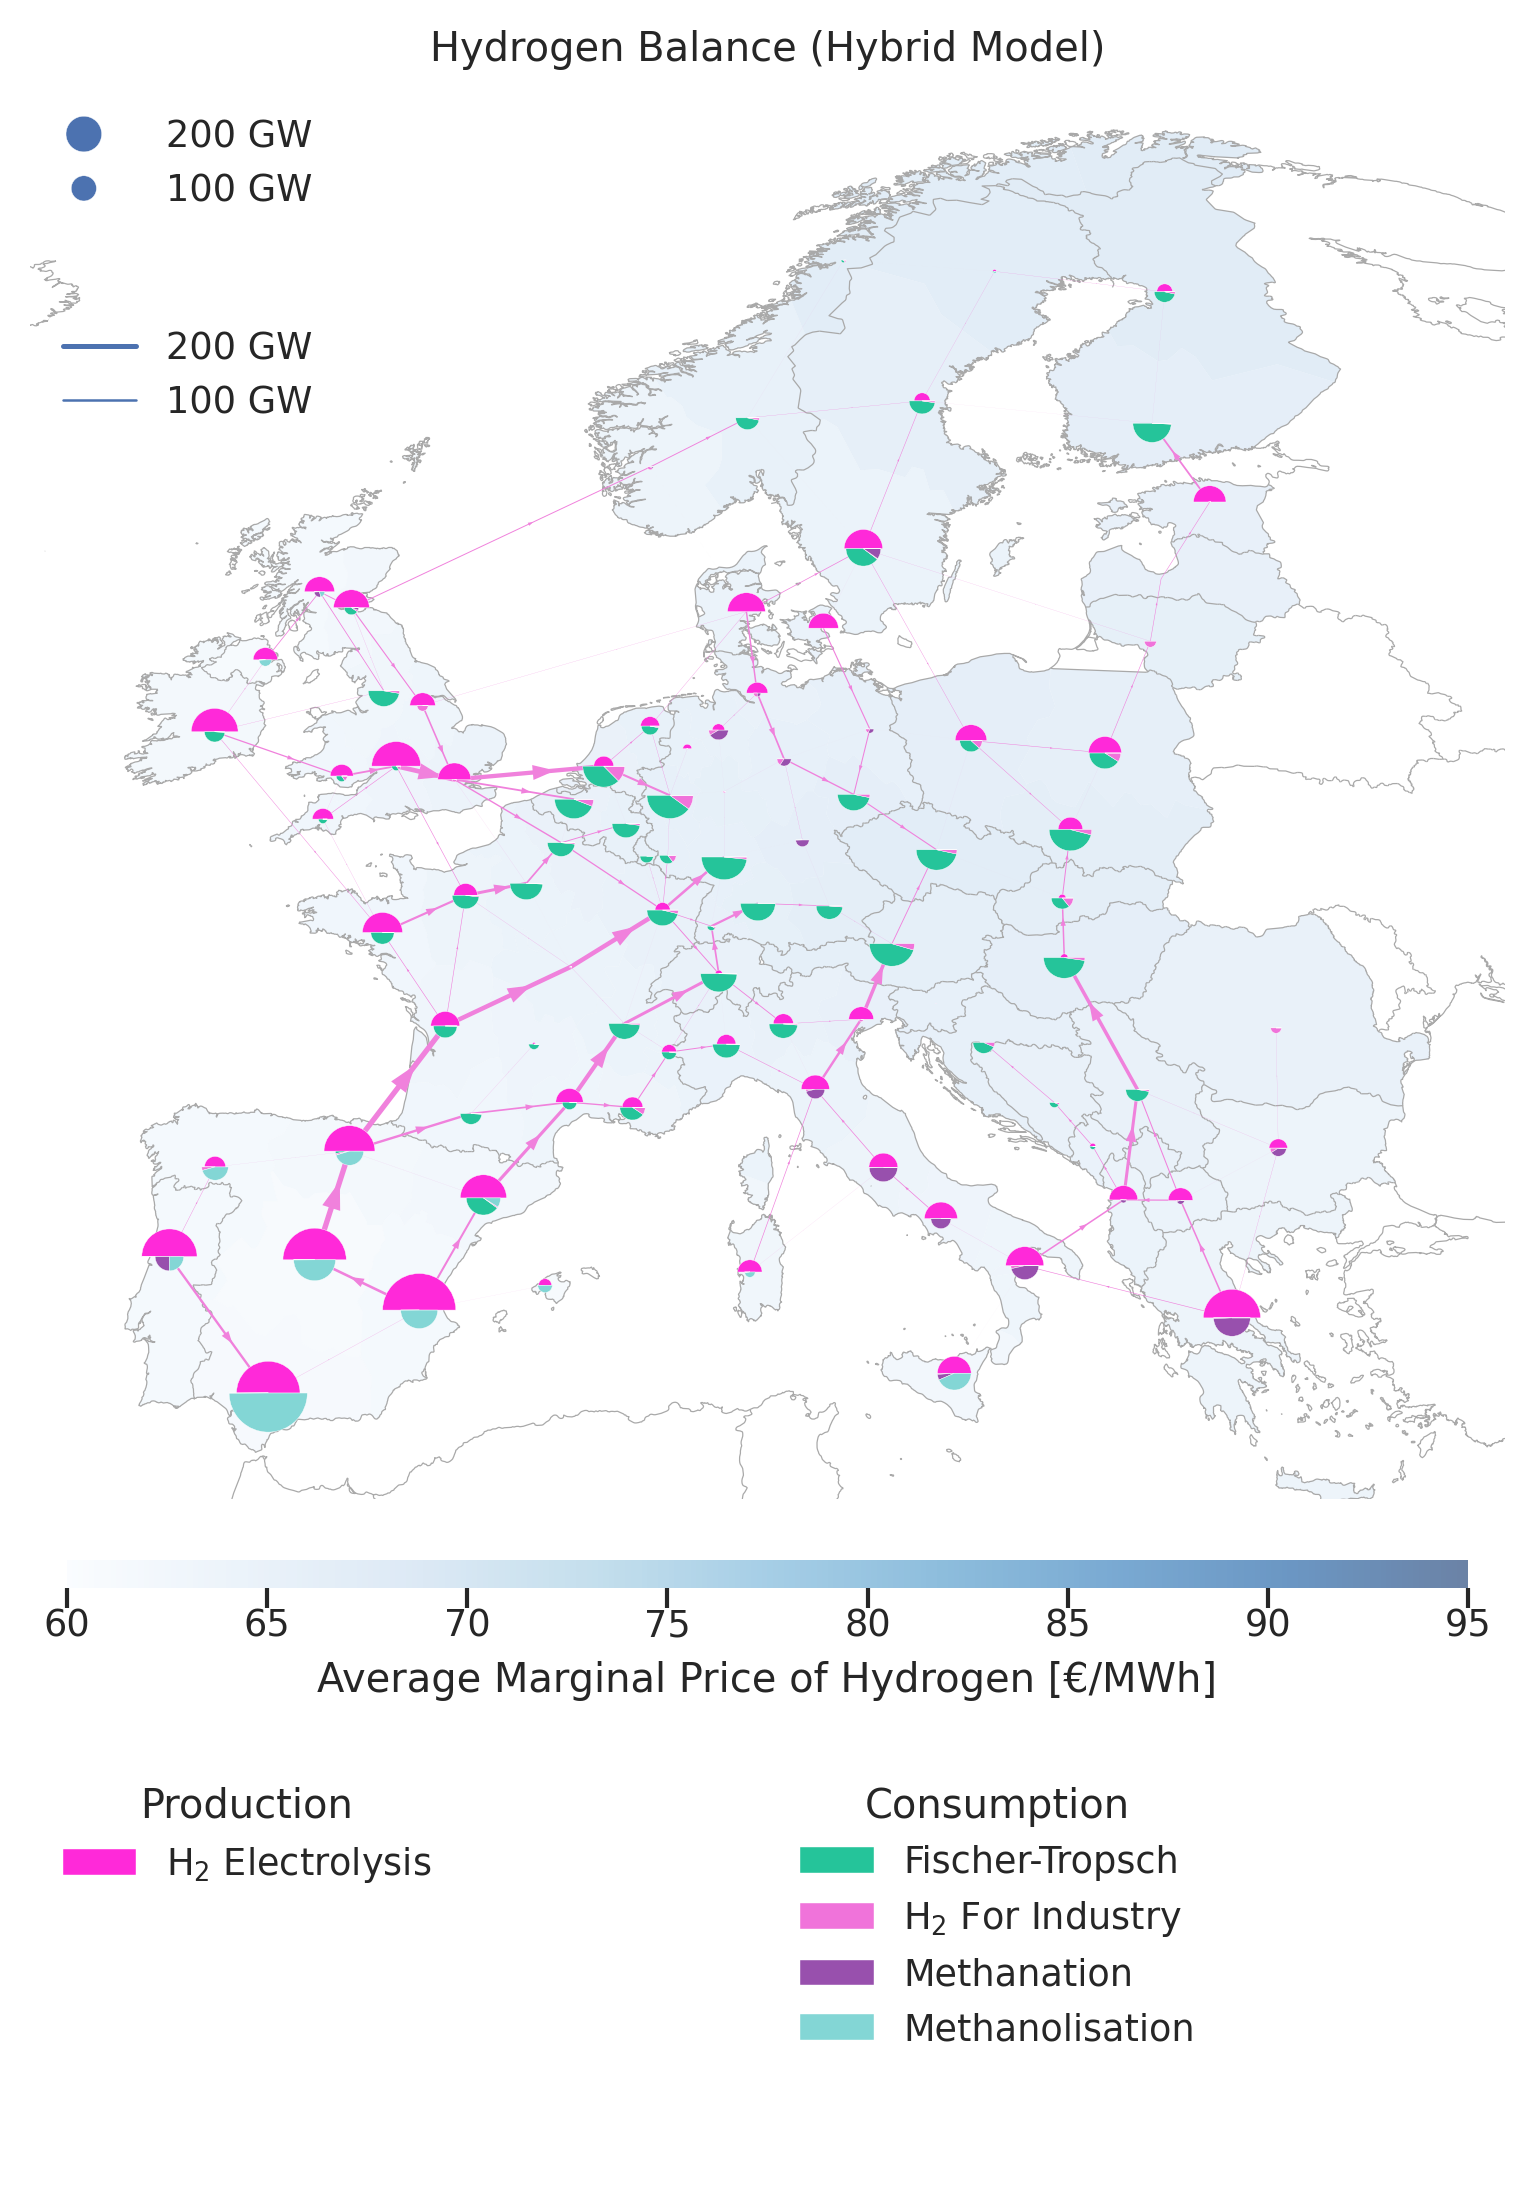
\includegraphics[width=0.35\textwidth]{other/carbon_networks_balance_map_hydrogen}

  \source{Hofmann, Tries, Neumann, Zeyen, Brown, 2024; \url{https://arxiv.org/abs/2402.19042}}

\end{frame}


\begin{frame}{\textbf{Carbon management}: Capture, use, transport and sequestration}
  
  \begin{center}
    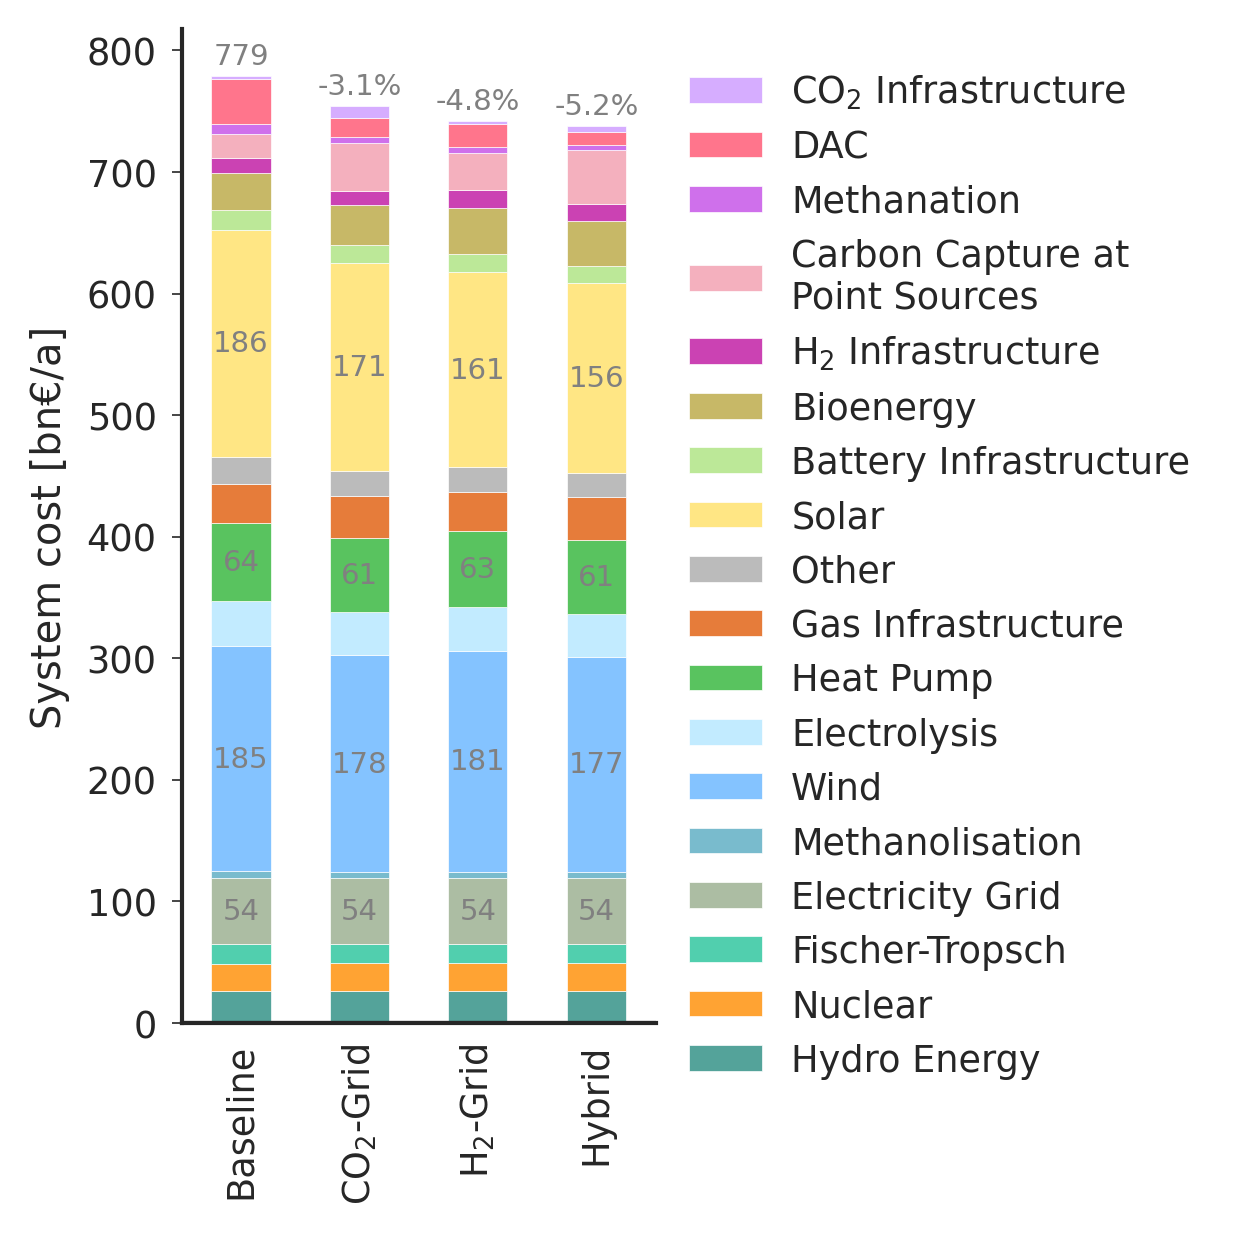
\includegraphics[height=0.73\textheight]{other/carbon_networks_cost_bar}
    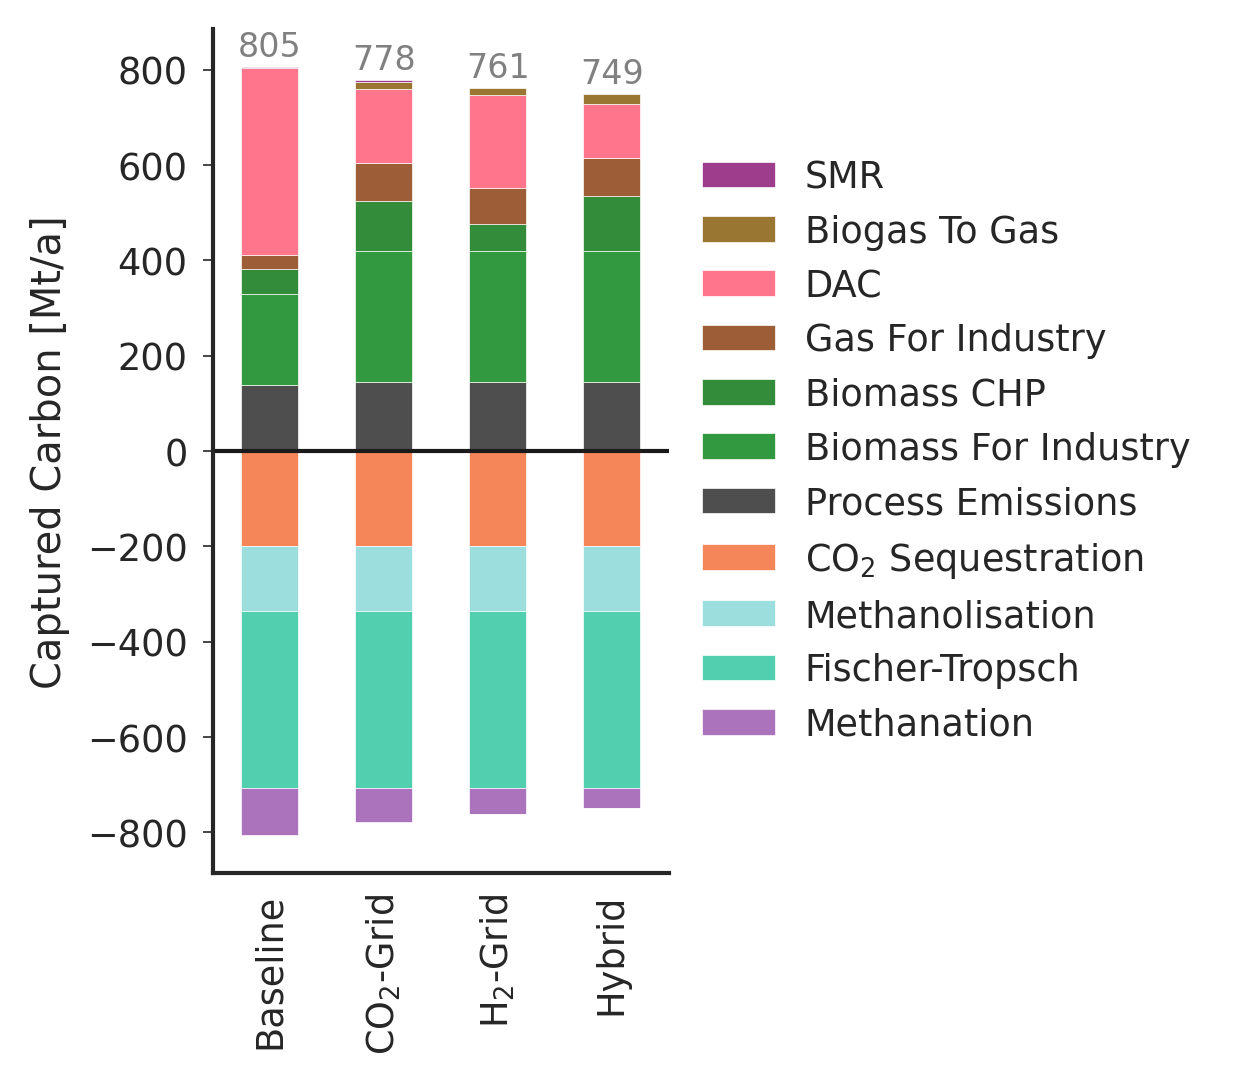
\includegraphics[height=0.71\textheight]{other/carbon_networks_balance_bar_carbon}

    \footnotesize
    \begin{itemize}
      \item \alert{CCS} for process emissions (for instance, in cement industry)
      \item \alert{CCU} for e-synfuels and e-chemicals (in particular, shipping, aviation, plastics)
      \item \alert{CDR} for unabatable and negative emissions (to offset imperfect capture rates)
    \end{itemize}

  \end{center}

  \source{Hofmann, Tries, Neumann, Zeyen, Brown, 2024; \url{https://arxiv.org/abs/2402.19042}}

\end{frame}

\end{document}